\begin{frame}[fragile]{Tutorial: One-site operators}

\begin{columns}

\begin{column}{4.5cm}

\begin{onlyenv}<1->
\begin{lstlisting}[language=JuliaLocal, style=julia, basicstyle=\small]
Z = ITensor(i', i)
Z[i'=>1, i=>1] = 1
Z[i'=>2, i=>2] = -1
\end{lstlisting}
\end{onlyenv}

\begin{onlyenv}<3->
\begin{lstlisting}[language=JuliaLocal, style=julia, basicstyle=\small]
z = [
  1 0
  0 -1
]
Z = ITensor(z, i', dag(i))


Z = op("Z", i)
\end{lstlisting}
\end{onlyenv}

\end{column}

\begin{column}{4.5cm}

\begin{onlyenv}<1-1>
$Z = \begin{bmatrix} 1 & 0 \\ 0 & -1 \end{bmatrix}$
\end{onlyenv}

\begin{onlyenv}<2->
\begin{center}
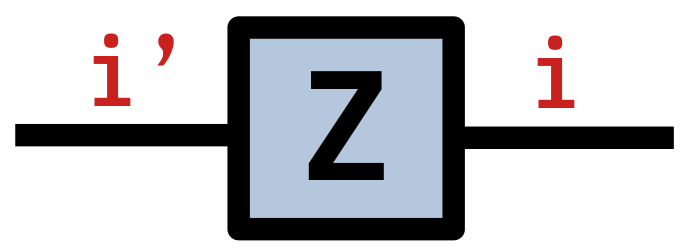
\includegraphics[width=0.6\textwidth]{
  slides/assets/Z.png
}
\end{center}
\vspace*{0.5cm}
\end{onlyenv}

\begin{onlyenv}<3->
Matrix representation Z \\
~\\
~\\
~\\
Convert to ITensor \\
~\\
~\\
Use predefined definition
\end{onlyenv}

\end{column}

\end{columns}

\end{frame}
